\documentclass[12pt]{article}
\usepackage[UTF8]{ctex}
\usepackage{geometry}
\usepackage{listings}
\usepackage{graphicx}
\usepackage{subfigure}
\usepackage{array}
\usepackage{caption}    
\usepackage{float}
\usepackage{hyperref}

\geometry{left=15mm,right=15mm,top=20mm,bottom=20mm}
\ctexset{today=old}
\ctexset{bibname=Reference}
\title{Report of Homework 1}
\author{PB21010362 汪兆辰}
\date{\today}

\begin{document}
\maketitle

\section{The Instruction of the Program File}
The Program includes a header file and a main program. In the header file "matrix.h", two objects, Matrix and SparseMatrix are defined.
The main program contains some test datas.

\subsection{Matrix}
The object Matrix is stored as a linear array. Using the function "Map" to find the location of a given element, which receives a coordinate and returns an integer. 
For users to visit the value of certain coordinate, the operator brackets and square brackets are defined, but actually what they do is invoking the function "Map":
\begin{lstlisting}
    inline int Map(int r,int c) const {
        if(r>rows||r<=0||c<=0||c>cols) { 
            throw out_of_range("Out of Range!");
        }
        return (r-1)*cols+c-1;
    }
\end{lstlisting}

The class contains the overload of operators. Here we just use the addition of matrix as an example, as the algorithms of other operators are actully similar. 
\begin{lstlisting}
    Matrix operator+ (const Matrix& rhs) {
        if(rhs.cols!=cols||rhs.rows!=rows){
            throw logic_error("Size mismatch");
        }
        Matrix Mt(rows,cols);
        for(int i=0;i<rows;i++){
            for(int j=0;j<cols;j++){
                Mt.data[Map(i+1,j+1)]=rhs.data[Map(i+1,j+1)]
                +data[Map(i+1,j+1)];
            }
        }
        return Mt;
    }
\end{lstlisting}
The matrix Mt is used for returning the result of addition. The value of each element in Mt is the sum of rhs and *this at the same location. After walking through the two martrixs, we get the sum 
of the two and return it in Mt.

\subsection{SparseMatrix}
The SparseMatrix is stored as a linked-list, which contains all the nonzero elements. The type of nodes is defined as Node, which includes the row, column and the value of the element. The head of the list is defined by the parameter {(-1,-1,0)}. 
In the constructor, an array of Node* is create, and for every row of the matrix, the head node is created.
\begin{lstlisting}
    SparseMatrix(int row,int col):rows(row),cols(col){
        matrix=new Node*[row+1];
        for(int i=1;i<=rows;i++){
            matrix[i]=new Node(-1,-1,0);
        }
    }
\end{lstlisting}

To change the value of element, the function "{add-element}" is defined. It finds the given place and insert the new node into the list. 
\begin{lstlisting}
    void add_element(int r,int c,R v){
        if(v==0)return;

        Node* p=matrix[r];
        while(p->next&&p->next->Col<c){
            p=p->next;
        }
        if(p->next&&p->next->Col==c){
            p->next->Data=v;
        }
        else {
            auto new_node= new Node(r,c,v);
            new_node->next=p->next;
            p->next=new_node;
        }
    }
\end{lstlisting}

The algorithm of the addition is to merge the same location of the two matrixs. When one row of the matrix has been walked through, the rest of the other 
matrix are just put into the result matrix.
\begin{lstlisting}
    SparseMatrix operator+(const SparseMatrix& rhs){
        if(rows!=rhs.rows||cols!=rhs.cols){
            throw logic_error("Size mismatch");
        }
        SparseMatrix result(rows,cols);
        for(int r=1;r<=rows;r++){
            Node* p1=matrix[r]->next;
            Node* p2=rhs.matrix[r]->next;

            while(p1&&p2){//merge the element at the same location
                if(p1->Col < p2->Col){
                    result.add_element(p1->Row,p1->Col,p1->Data);
                    p1=p1->next;
                }
                else if(p1->Col > p2->Col){
                    result.add_element(p2->Row,p2->Col,p2->Data);
                    p2=p2->next;
                }
                else {
                    result.add_element(p1->Row,p1->Col,p1->Data+p2->Data);
                    p1=p1->next;
                    p2=p2->next;
                }
            }
            //add the rest of the elements
            while(p1){
                result.add_element(p1->Row,p1->Col,p1->Data);
                p1=p1->next;
            }
            while(p2){
                result.add_element(p2->Row,p2->Col,p2->Data);
                p2=p2->next;
            }

        }
        return result;
    }
\end{lstlisting}

\section{Test and Result}
\subsection{Fill Matrix with random numbers}
Fill two matrixs with random numbers and add them up. The running results are as follows:
\begin{figure}[H]
    \centering
    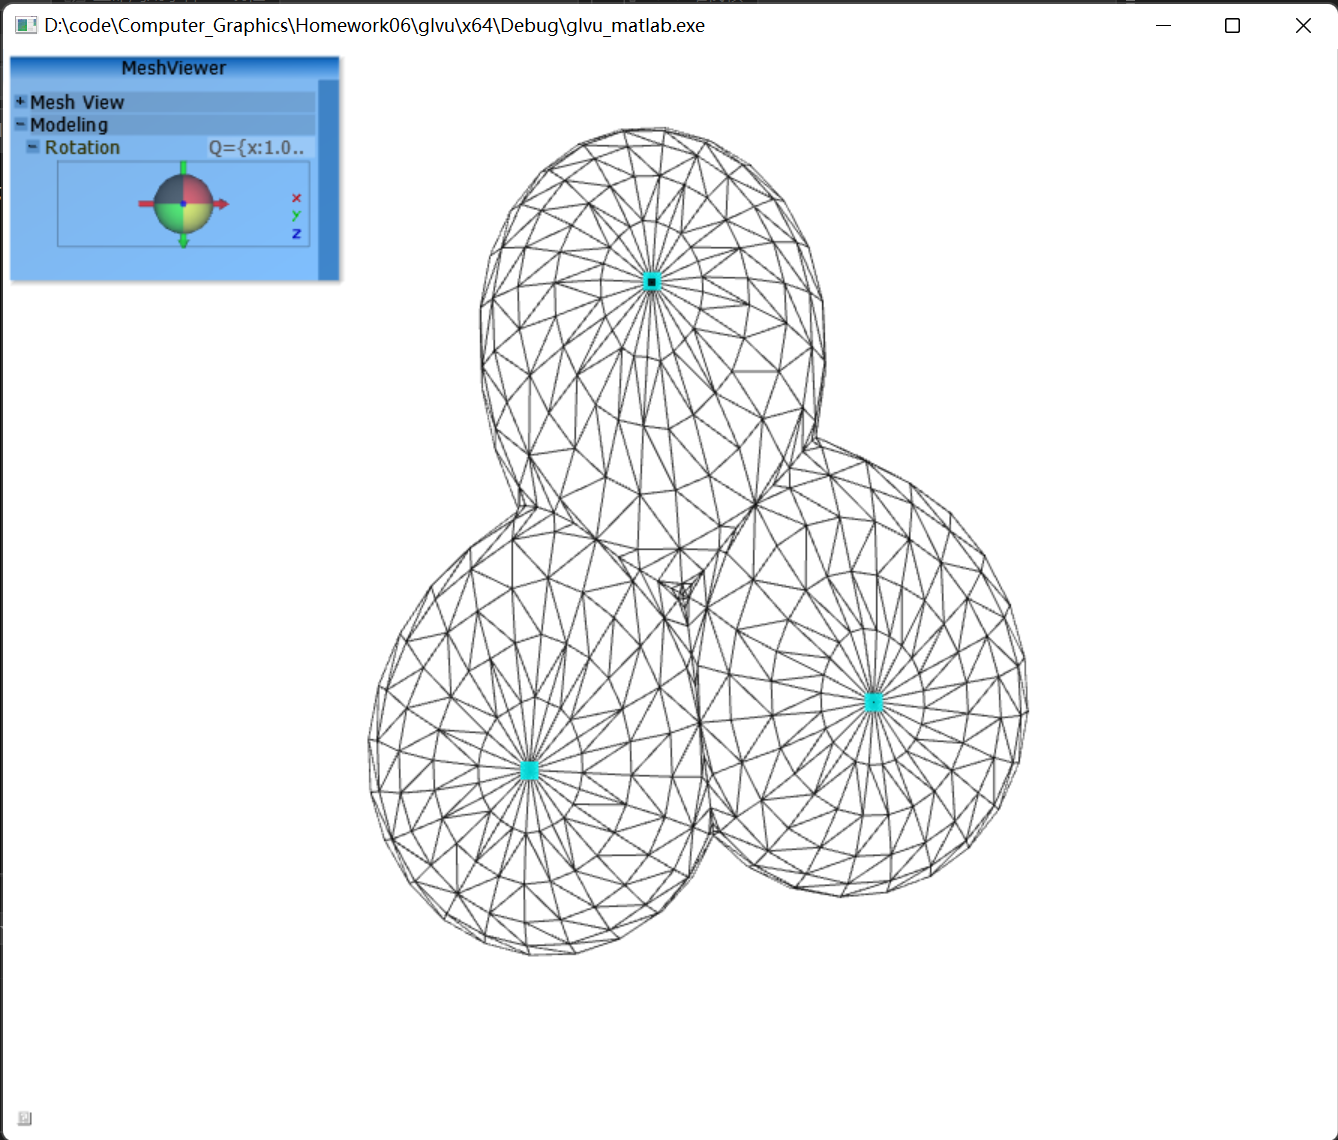
\includegraphics[scale=0.9]{pic1.png}
\end{figure}

\subsection{Benchmark with runtime}
Using the lib chrono. Get the start time and end time of the program, by comparing the two time we get the duration 
of certain command.The codes are as follows:
\begin{lstlisting}
    auto start_time=chrono::system_clock::now();
    Matrix<double> C = A*B;
    auto end_time=chrono::system_clock::now();
    auto duration = chrono::duration_cast<chrono::milliseconds>
    (end_time - start_time);
    double time_in_milliseconds = static_cast<double>(duration.count());
\end{lstlisting}
To make the duration long enough, we enlarge the scale of matrixs into {(2000*2000)}, and use chrono to get the duration of 
the multiplication of two matrixs. The running results are as follows:
\begin{figure}[H]
    \centering
    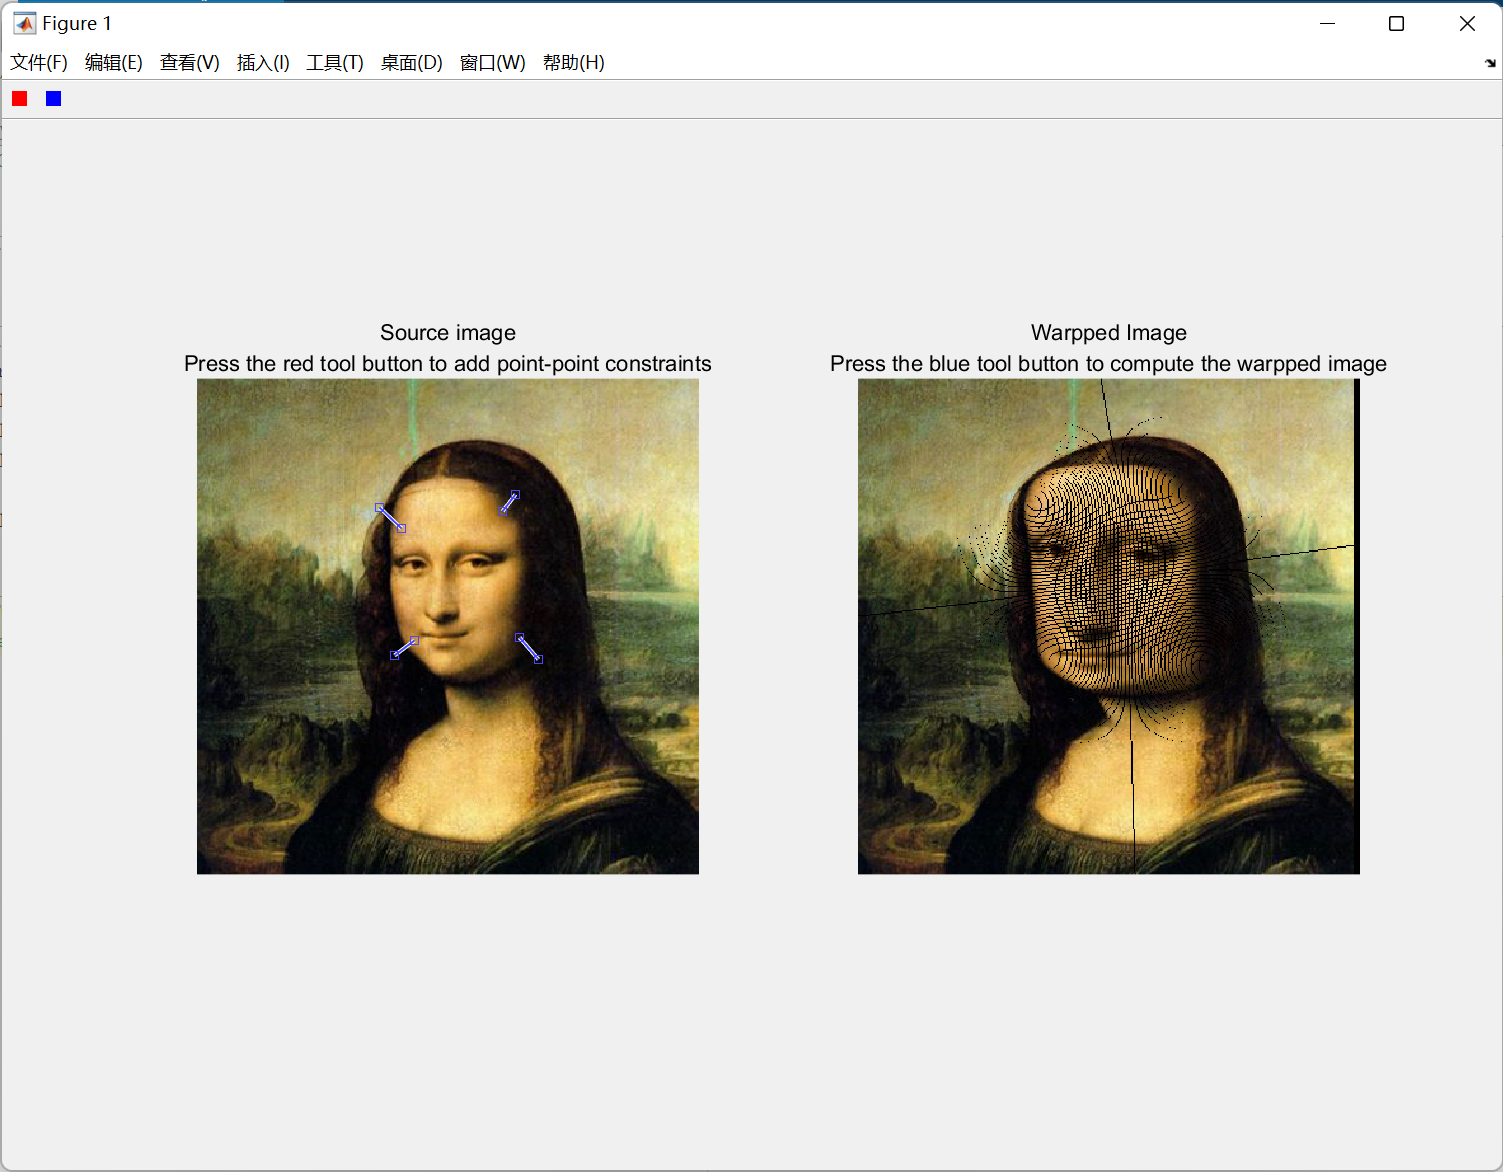
\includegraphics{pic2.png}
\end{figure}

\subsection{Compare with Eigen}
Using the lib Eigen and self-defined class Matrix to assign and operate matrixs.The test codes are as follows:
\begin{figure}[H]
    \centering
    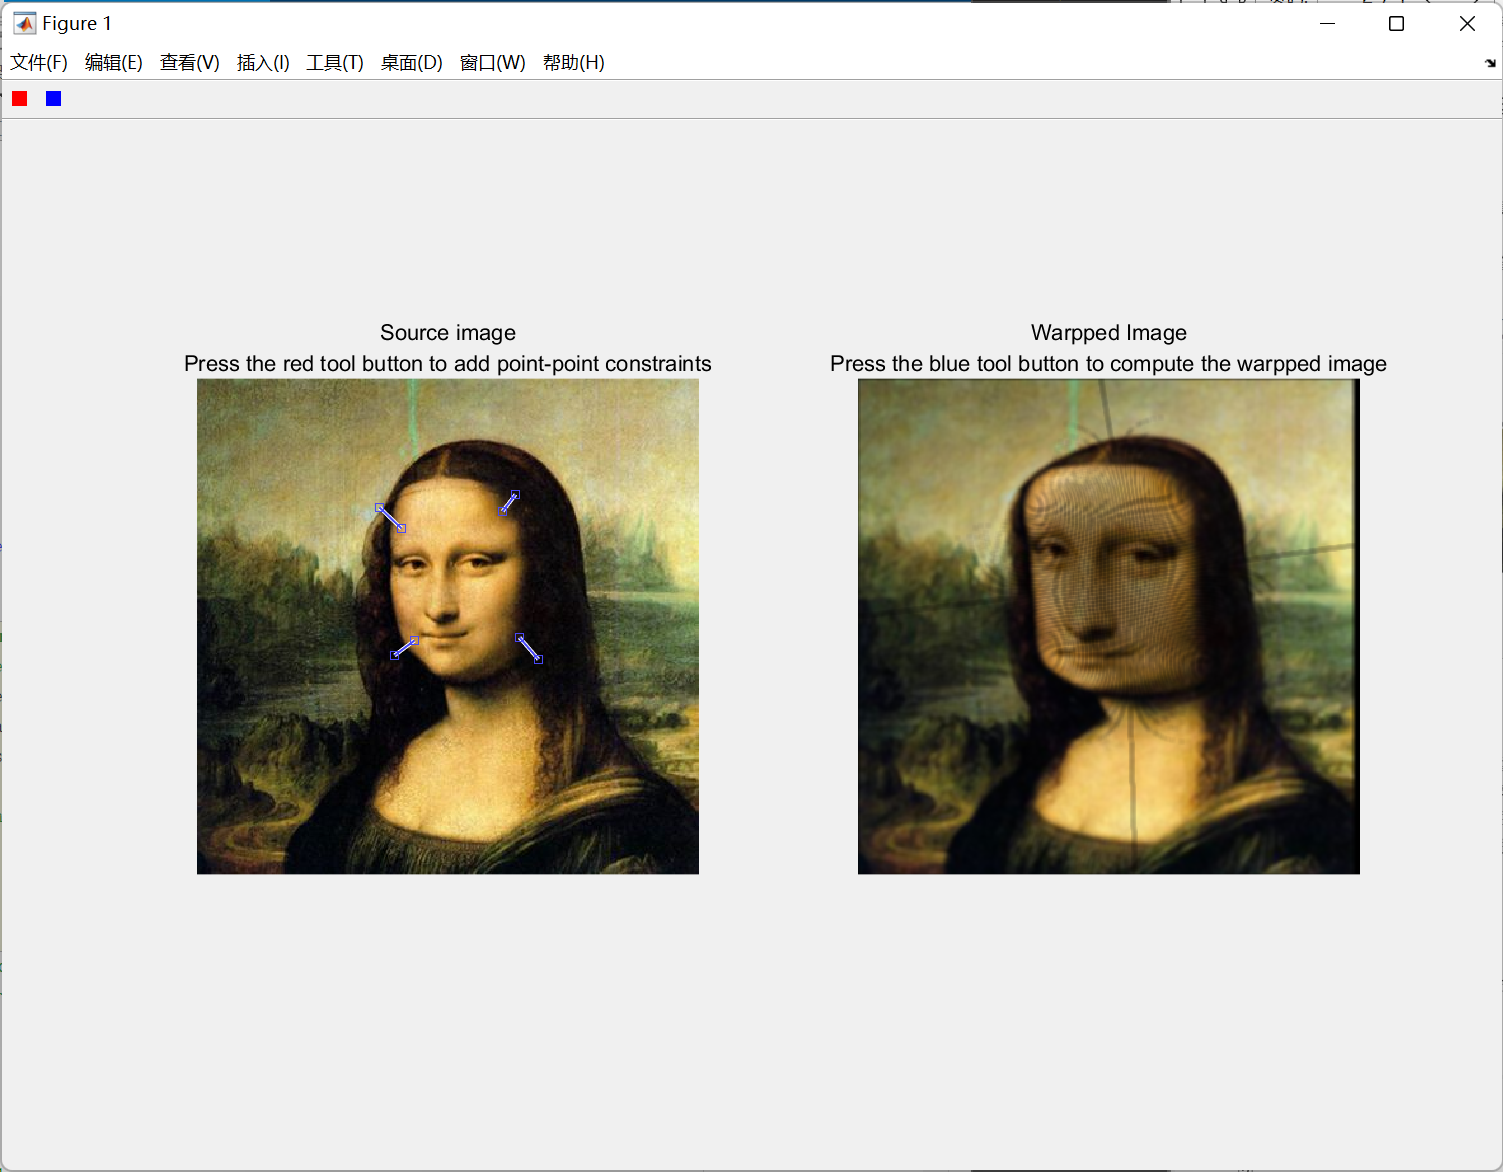
\includegraphics{pic3.png}
\end{figure}
the running results are as follows:
\begin{figure}[H]
    \centering
    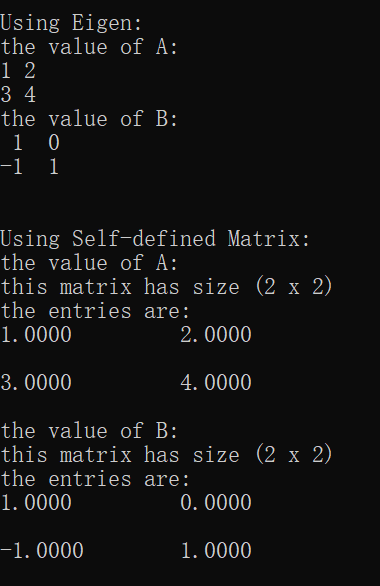
\includegraphics{pic4.png}
\end{figure}

\subsection{Test of SparseMatrix}
Test the assignment, addition and printing of sparse matrixs.Test code are as follows:
\begin{figure}[H]
    \centering
    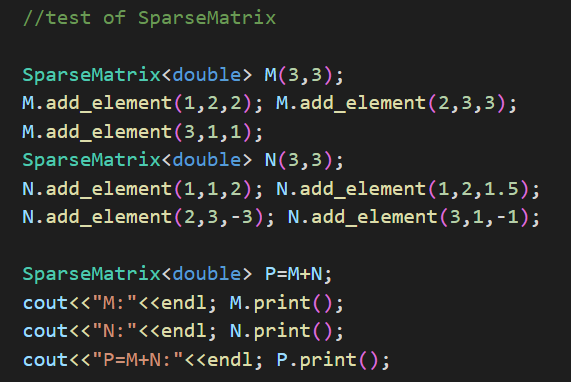
\includegraphics{pic5.png}
\end{figure}
the running results are as follows:
\begin{figure}[H]
    \centering
    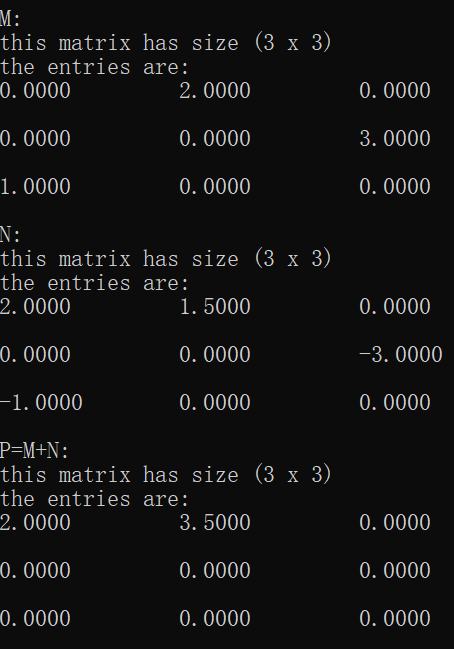
\includegraphics{pic6.png}
\end{figure}

\begin{thebibliography}{1}
    \bibitem{S} Stephen Prata. C++ Primer Plus. Beijing: People Telecom Press, 2012.
    \bibitem{c1} \url{https://blog.csdn.net/qq_36336522/article/details/79410813}
    \bibitem{c2} \url{https://blog.csdn.net/qq_45797026/article/details/108536921}
    \bibitem{z} \url{https://zhuanlan.zhihu.com/p/462494086}
\end{thebibliography}
    

\end{document}
